\documentclass[12pt,letterpaper]{article}
\usepackage{graphicx,textcomp}
\usepackage{natbib}
\usepackage{setspace}
\usepackage{fullpage}
\usepackage{color}
\usepackage[reqno]{amsmath}
\usepackage{amsthm}
\usepackage{fancyvrb}
\usepackage{amssymb,enumerate}
\usepackage[all]{xy}
\usepackage{endnotes}
\usepackage{lscape}
\newtheorem{com}{Comment}
\usepackage{float}
\usepackage{hyperref}
\newtheorem{lem} {Lemma}
\newtheorem{prop}{Proposition}
\newtheorem{thm}{Theorem}
\newtheorem{defn}{Definition}
\newtheorem{cor}{Corollary}
\newtheorem{obs}{Observation}
\usepackage[compact]{titlesec}
\usepackage{dcolumn}
\usepackage{tikz}
\usetikzlibrary{arrows}
\usepackage{multirow}
\usepackage{xcolor}
\newcolumntype{.}{D{.}{.}{-1}}
\newcolumntype{d}[1]{D{.}{.}{#1}}
\definecolor{light-gray}{gray}{0.65}
\usepackage{url}
\usepackage{listings}
\usepackage{color}

\definecolor{codegreen}{rgb}{0,0.6,0}
\definecolor{codegray}{rgb}{0.5,0.5,0.5}
\definecolor{codepurple}{rgb}{0.58,0,0.82}
\definecolor{backcolour}{rgb}{0.95,0.95,0.92}

\lstdefinestyle{mystyle}{
	backgroundcolor=\color{backcolour},   
	commentstyle=\color{codegreen},
	keywordstyle=\color{magenta},
	numberstyle=\tiny\color{codegray},
	stringstyle=\color{codepurple},
	basicstyle=\footnotesize,
	breakatwhitespace=false,         
	breaklines=true,                 
	captionpos=b,                    
	keepspaces=true,                 
	numbers=left,                    
	numbersep=5pt,                  
	showspaces=false,                
	showstringspaces=false,
	showtabs=false,                  
	tabsize=2
}
\lstset{style=mystyle}
\newcommand{\Sref}[1]{Section~\ref{#1}}
\newtheorem{hyp}{Hypothesis}

\title{Problem Set 3}
\date{Due: November 12, 2026}
\author{Ella Lang}


\begin{document}
	\maketitle
	\section*{Instructions}
	\begin{itemize}
		\item Please show your work! You may lose points by simply writing in the answer. If the problem requires you to execute commands in \texttt{R}, please include the code you used to g\\
		et your answers. Please also include the \texttt{.R} file that contains your code. If you are not sure if work needs to be shown for a particular problem, please ask.
	\item Your homework should be submitted electronically on GitHub.
	\item This problem set is due before 23:59 on Thursday November 12, 2026. No late assignments will be accepted.

	\end{itemize}

		\vspace{.25cm}
	
\noindent In this problem set, you will run several regressions and create an add variable plot (see the lecture slides) in \texttt{R} using the \texttt{incumbents\_subset.csv} dataset. Include all of your code.

	\vspace{.5cm}
\section*{Question 1}
\vspace{.25cm}
\noindent We are interested in knowing how the difference in campaign spending between incumbent and challenger affects the incumbent's vote share. 
	\begin{enumerate}
		\item Run a regression where the outcome variable is \texttt{voteshare} and the explanatory variable is \texttt{difflog}.	
		\lstinputlisting[language=R, firstline=35, lastline=36]{PS03_answers_el.la.R} 
		\lstinputlisting[language=R, firstline=41, lastline=42]{PS03_answers_el.la.R}  
		\noindent I first checked the summary of both variables to confirm they were numerical and didn't require any changes such as factorization. I then used the lm() function to run a regression with voteshare as the outcome variable and difflog as the explanatory variable. I also used the stargazer function from the stargazer package to provide an output suitable for texstudio, shown in table 1. The same process was used for each of the linear regressions run below. \\
		\newpage
		\begin{table}[!htbp] \centering 
			\caption{} 
			\label{} 
			\begin{tabular}{@{\extracolsep{5pt}}lc} 
				\\[-1.8ex]\hline 
				\hline \\[-1.8ex] 
				& \multicolumn{1}{c}{\textit{Dependent variable:}} \\ 
				\cline{2-2} 
				\\[-1.8ex] & Vote Share \\ 
				\hline \\[-1.8ex] 
				Difference in Campaign Spending & 0.042$^{***}$ \\ 
				& (0.001) \\ 
				& \\ 
				Constant & 0.579$^{***}$ \\ 
				& (0.002) \\ 
				& \\ 
				\hline \\[-1.8ex] 
				Observations & 3,193 \\ 
				R$^{2}$ & 0.367 \\ 
				Adjusted R$^{2}$ & 0.367 \\ 
				Residual Std. Error & 0.079 (df = 3191) \\ 
				F Statistic & 1,852.791$^{***}$ (df = 1; 3191) \\ 
				\hline 
				\hline \\[-1.8ex] 
				\textit{Note:}  & \multicolumn{1}{r}{$^{*}$p$<$0.1; $^{**}$p$<$0.05; $^{***}$p$<$0.01} \\ 
			\end{tabular} 
		\end{table} 
		\noindent For each unit increase in the log difference between campaign spending for incumbent and challenger, on average there is a 0.042 increase in vote share for the incumbent. When there is no difference in campaign spending between incumbent and challenger, there incumbent is predicted to receive 0.579 of the vote share. The R$^{2}$ is 0.367, meaning difference in campaign spending accounts for 36.7\% of the variation in incumbent vote share. \\
		\item Make a scatterplot of the two variables and add the regression line. 	
		\lstinputlisting[language=R, firstline=46, lastline=52]{PS03_answers_el.la.R} 
		\newpage 
		\begin{figure}[h!]\centering
			\label{fig:plot_1}
			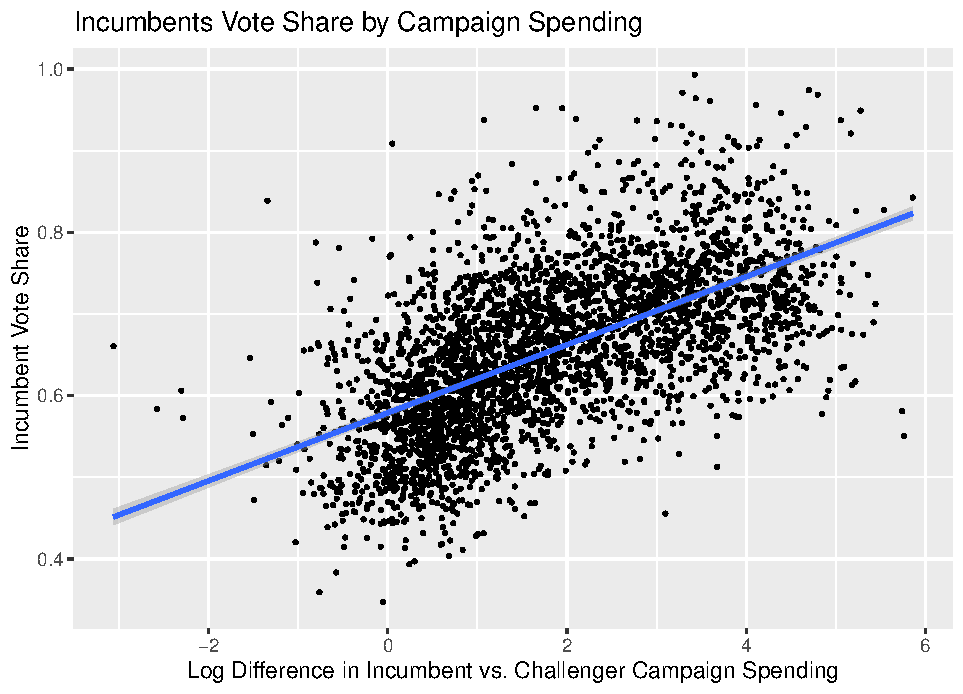
\includegraphics[width=.75\textwidth]{Rplot06.pdf}
		\end{figure}
		\noindent The scatterplot shows a moderate positive correlation between incumbent campaign spending compared to challenger and incumbent vote share. This means that an increase in the difference between incumbent and challenger spending (when the incumbent is spending more) is associated with an increase in the incumbent's vote share. The data points are mostly clustered between 0 and 5 on the x-axis meaning incumbents most often spend more than challengers. The data points are also widely spread around the line, indicating that much of the variation in vote share is not explained by campaign spending. \\
		\item Save the residuals of the model in a separate object.
		\lstinputlisting[language=R, firstline=56, lastline=56]{PS03_answers_el.la.R} 
		\item Write the prediction equation.
		\begin{equation}
			\hat{y} = b_0 + b_1 x
		\end{equation}
		\begin{equation}
			\widehat{voteshare} = 0.579 + 0.042 \times  \text{difflog}
		\end{equation}
	\end{enumerate}
	

\section*{Question 2}
\noindent We are interested in knowing how the difference between incumbent and challenger's spending and the vote share of the presidential candidate of the incumbent's party are related.	\vspace{.1cm}
	\begin{enumerate}
		\item Run a regression where the outcome variable is \texttt{presvote} and the explanatory variable is \texttt{difflog}.
		\lstinputlisting[language=R, firstline=37,lastline=37]{PS03_answers_el.la.R}
		\lstinputlisting[language=R, firstline=60,lastline=62]{PS03_answers_el.la.R}
		\noindent I checked the summary of the presvote variable to confirm it was numerical and didn't require any changes such as factorization, then ran the linear regression. \\
		
		\begin{table}[!htbp] \centering 
			\caption{} 
			\label{} 
			\begin{tabular}{@{\extracolsep{5pt}}lc} 
				\\[-1.8ex]\hline 
				\hline \\[-1.8ex] 
				& \multicolumn{1}{c}{\textit{Dependent variable:}} \\ 
				\cline{2-2} 
				\\[-1.8ex] & Presidential Vote Share \\ 
				\hline \\[-1.8ex] 
				Difference in Campaign Spending & 0.024$^{***}$ \\ 
				& (0.001) \\ 
				& \\ 
				Constant & 0.508$^{***}$ \\ 
				& (0.003) \\ 
				& \\ 
				\hline \\[-1.8ex] 
				Observations & 3,193 \\ 
				R$^{2}$ & 0.088 \\ 
				Adjusted R$^{2}$ & 0.088 \\ 
				Residual Std. Error & 0.110 (df = 3191) \\ 
				F Statistic & 307.715$^{***}$ (df = 1; 3191) \\ 
				\hline 
				\hline \\[-1.8ex] 
				\textit{Note:}  & \multicolumn{1}{r}{$^{*}$p$<$0.1; $^{**}$p$<$0.05; $^{***}$p$<$0.01} \\ 
			\end{tabular} 
		\end{table}
		\noindent For each unit increase in the log difference between campaign spending of incumbent and challenger, on average, there is a 0.024 increase in vote share of the presidential candidate of the incumbent's party. When there is no difference between campaign spending between the incumbent and challenger, the vote share of the presidential candidate of the incumbent's party is expected to be 0.508. The R$^{2}$ is 0.088, meaning difference in campaign spending accounts for 8.8\% of the variation in presidential vote share.\\
		\item Make a scatterplot of the two variables and add the regression line. 
		\lstinputlisting[language=R, firstline=65,lastline=71]{PS03_answers_el.la.R}
		\newpage 
		\begin{figure}[h!]\centering
			\label{fig:plot_1}
			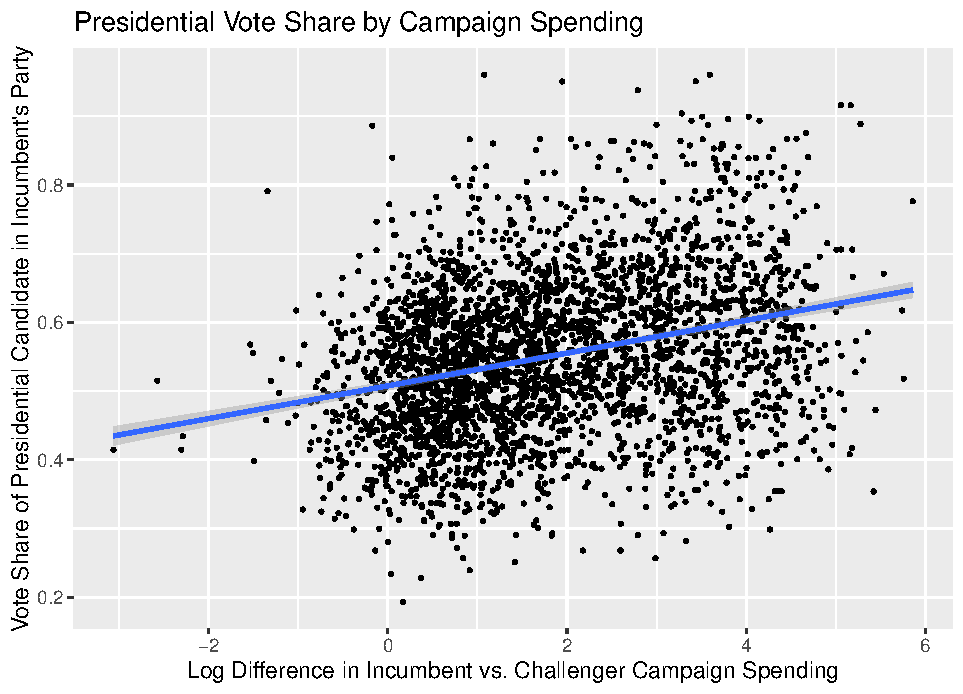
\includegraphics[width=.85\textwidth]{Rplot07.pdf}
		\end{figure}
		\noindent I used the ggplot2 package to create a scatterplot with a regression line. The scatterplot shows a weak positive correlation between campaign spending and vote share of presidential candidate of the incumbent's party. This means that an increase in the difference between incumbent and challenger spending (when the incumbent is spending more) is associated with a slight increase in the vote share of presidential candidates in the incumbent's party. The data points are widely distributed around the line, suggesting that much of the variation in presidential vote share is not accounted for by campaign spending.  \\
		\item Save the residuals of the model in a separate object.	
		\lstinputlisting[language=R, firstline=75,lastline=75]{PS03_answers_el.la.R}
		\item Write the prediction equation.
		\begin{equation}
			\hat{y} = b_0 + b_1 x
		\end{equation}
		\begin{equation}
			\widehat{presvote} = 0.508 + 0.024 \times  \text{difflog}
		\end{equation}
	\end{enumerate}
	
		
\section*{Question 3}

\noindent We are interested in knowing how the vote share of the presidential candidate of the incumbent's party is associated with the incumbent's electoral success.
	\vspace{.25cm}
	\begin{enumerate}
		\item Run a regression where the outcome variable is \texttt{voteshare} and the explanatory variable is \texttt{presvote}.
		\lstinputlisting[language=R, firstline=79,lastline=80]{PS03_answers_el.la.R}
		\begin{table}[!htbp] \centering 
			\caption{} 
			\label{} 
			\begin{tabular}{@{\extracolsep{5pt}}lc} 
				\\[-1.8ex]\hline 
				\hline \\[-1.8ex] 
				& \multicolumn{1}{c}{\textit{Dependent variable:}} \\ 
				\cline{2-2} 
				\\[-1.8ex] & Vote Share \\ 
				\hline \\[-1.8ex] 
				Presidential Vote Share & 0.388$^{***}$ \\ 
				& (0.013) \\ 
				& \\ 
				Constant & 0.441$^{***}$ \\ 
				& (0.008) \\ 
				& \\ 
				\hline \\[-1.8ex] 
				Observations & 3,193 \\ 
				R$^{2}$ & 0.206 \\ 
				Adjusted R$^{2}$ & 0.206 \\ 
				Residual Std. Error & 0.088 (df = 3191) \\ 
				F Statistic & 826.950$^{***}$ (df = 1; 3191) \\ 
				\hline 
				\hline \\[-1.8ex] 
				\textit{Note:}  & \multicolumn{1}{r}{$^{*}$p$<$0.1; $^{**}$p$<$0.05; $^{***}$p$<$0.01} \\ 
			\end{tabular} 
		\end{table} 
		\noindent For each unit increase in the vote share of the presidential candidate of incumbents party's, on average, there is a 0.388 increase in incumbent's vote share. The intercept term is 0.441, but as it is highly unlikely that the presidential candidate would have a vote share of 0 this is not theoretically useful. The R$^{2}$ is 0.206, meaning that presidential vote share accounts for 20.6\% of the variation in incumbent vote share.\\
		\item Make a scatterplot of the two variables and add the regression line. 
		\lstinputlisting[language=R, firstline=84,lastline=90]{PS03_answers_el.la.R}
		\begin{figure}[h!]\centering
			\label{fig:plot_1}
			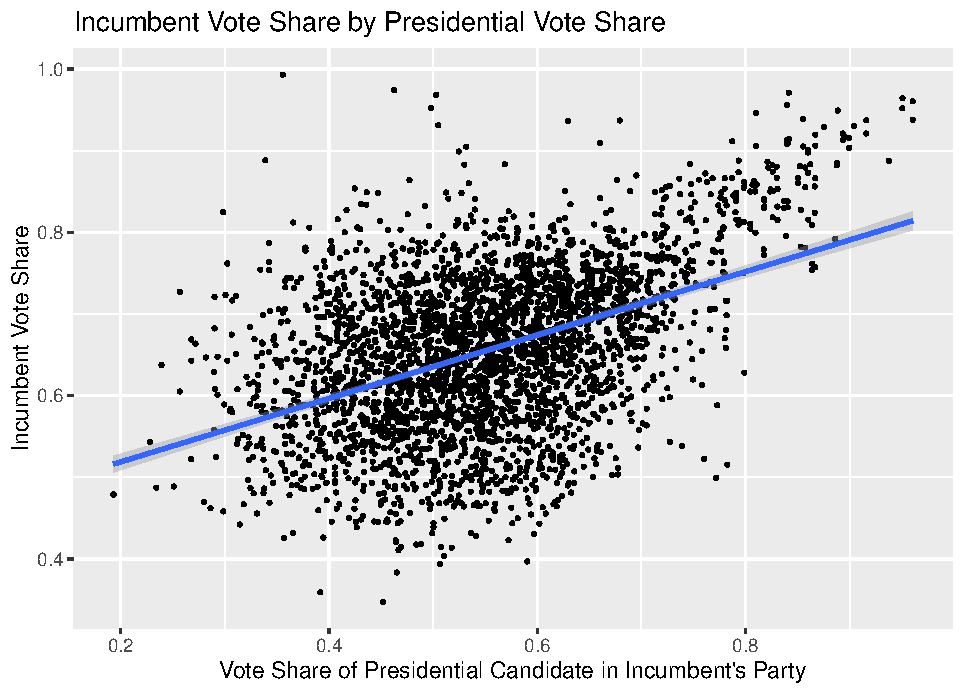
\includegraphics[width=.85\textwidth]{Rplot08.pdf}
		\end{figure}
		\noindent The scatterplot shows a moderate positive correlation between vote share of presidential candidate in incumbents party and incumbent vote share. This means that an increase in the vote share of the presidential candidate in the incumbent's party is associated with an increase in the incumbent's vote share. The data points are also widely scattered around the line, suggesting that much of the variation in incumbent vote share is unaccounted for by vote share of presidential candidate in incumbents party.\\
		\item Write the prediction equation.
		\begin{equation}
			\hat{y} = b_0 + b_1 x
		\end{equation}
		\begin{equation}
			\widehat{voteshare} = 0.441 + 0.388 \times  \text{presvote}
		\end{equation}
	\end{enumerate}
	

\newpage	
\section*{Question 4}
\noindent The residuals from part (a) tell us how much of the variation in \texttt{voteshare} is $not$ explained by the difference in spending between incumbent and challenger. The residuals in part (b) tell us how much of the variation in \texttt{presvote} is $not$ explained by the difference in spending between incumbent and challenger in the district.
	\begin{enumerate}
		\item Run a regression where the outcome variable is the residuals from Question 1 and the explanatory variable is the residuals from Question 2.
			\lstinputlisting[language=R, firstline=94,lastline=95]{PS03_answers_el.la.R}
		\begin{table}[!htbp] \centering 
			\caption{} 
			\label{} 
			\begin{tabular}{@{\extracolsep{5pt}}lc} 
				\\[-1.8ex]\hline 
				\hline \\[-1.8ex] 
				& \multicolumn{1}{c}{\textit{Dependent variable:}} \\ 
				\cline{2-2} 
				\\[-1.8ex] & Question 1 Residuals \\ 
				\hline \\[-1.8ex] 
				Question 2 Residuals & 0.257$^{***}$ \\ 
				& (0.012) \\ 
				& \\ 
				Constant & $-$0.000 \\ 
				& (0.001) \\ 
				& \\ 
				\hline \\[-1.8ex] 
				Observations & 3,193 \\ 
				R$^{2}$ & 0.130 \\ 
				Adjusted R$^{2}$ & 0.130 \\ 
				Residual Std. Error & 0.073 (df = 3191) \\ 
				F Statistic & 476.975$^{***}$ (df = 1; 3191) \\ 
				\hline 
				\hline \\[-1.8ex] 
				\textit{Note:}  & \multicolumn{1}{r}{$^{*}$p$<$0.1; $^{**}$p$<$0.05; $^{***}$p$<$0.01} \\ 
			\end{tabular} 
		\end{table} 
		\noindent Holding the log difference in campaign spending constant, on average, a one unit increase in the vote share of the presidential candidate in the incumbent's party is associated with a 0.257 increase in the incumbent's vote share. The R$^{2}$ is 0.130, meaning that when log difference in campaign spending is held constant, presidential vote share accounts for 10.3\% of the variation in incumbent vote share (compared to 20.6\% when campaign spending is not accounted for).\\
		\item Make a scatterplot of the two residuals and add the regression line. 
		\lstinputlisting[language=R, firstline=99,lastline=105]{PS03_answers_el.la.R}
		\begin{figure}[h!]\centering
			\label{fig:plot_1}
			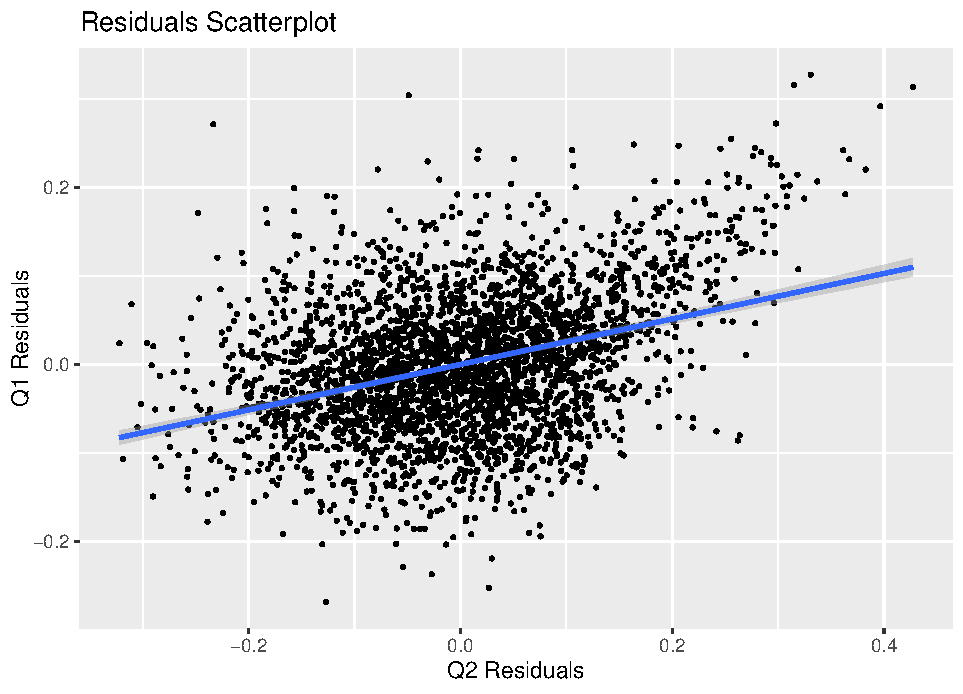
\includegraphics[width=.75\textwidth]{Rplot.pdf}
		\end{figure}
		\noindent Holding campaign spending constant, there is a weak to moderate positive correlation between vote share of the presidential candidate of the incumbents party and incumbent vote share. This means that when campaign spending is held constant, an increase in the vote share of the presidential candidate in the incumbent's party is still associated with an increase in the incumbent's vote share. \\
		\item Write the prediction equation.
		\begin{equation}
			\hat{y} = b_0 + b_1 x
		\end{equation}
		\begin{equation}
			\widehat{q1residuals} = -0.000 + 0.257 \times  \text{q2residuals}
		\end{equation}
	\end{enumerate}

\section*{Question 5}
\noindent What if the incumbent's vote share is affected by both the president's popularity and the difference in spending between incumbent and challenger? 
	\begin{enumerate}
		\item Run a regression where the outcome variable is the incumbent's \texttt{voteshare} and the explanatory variables are \texttt{difflog} and \texttt{presvote}.
		\lstinputlisting[language=R, firstline=109,lastline=110]{PS03_answers_el.la.R}
		\begin{table}[!htbp] \centering 
			\caption{} 
			\label{} 
			\begin{tabular}{@{\extracolsep{5pt}}lc} 
				\\[-1.8ex]\hline 
				\hline \\[-1.8ex] 
				& \multicolumn{1}{c}{\textit{Dependent variable:}} \\ 
				\cline{2-2} 
				\\[-1.8ex] & Vote Share \\ 
				\hline \\[-1.8ex] 
				Difference in Campaign Spending & 0.036$^{***}$ \\ 
				& (0.001) \\ 
				& \\ 
				Presidential Vote Share & 0.257$^{***}$ \\ 
				& (0.012) \\ 
				& \\ 
				Constant & 0.449$^{***}$ \\ 
				& (0.006) \\ 
				& \\ 
				\hline \\[-1.8ex] 
				Observations & 3,193 \\ 
				R$^{2}$ & 0.450 \\ 
				Adjusted R$^{2}$ & 0.449 \\ 
				Residual Std. Error & 0.073 (df = 3190) \\ 
				F Statistic & 1,302.947$^{***}$ (df = 2; 3190) \\ 
				\hline 
				\hline \\[-1.8ex] 
				\textit{Note:}  & \multicolumn{1}{r}{$^{*}$p$<$0.1; $^{**}$p$<$0.05; $^{***}$p$<$0.01} \\ 
			\end{tabular} 
		\end{table}	
		\noindent Holding presidential vote share constant, for each one unit increase in log difference in campaign spending, on average, there is a 0.36 increase in incumbent vote share. Holding log difference in campaign spending constant, for each unit increase in the vote share of the presidential candidate in the incumbent's party, on average there is a 0.257 increase in incumbent vote share. The R$^{2}$ is 0.450, meaning that presidential vote share and difference in campaign spending account for 45\% of the variation in incumbent vote share.\\
		\item Write the prediction equation.
		\begin{equation}
			\hat{y} = b_0 + b_1 x + b_2 x
		\end{equation}	
		\begin{equation}
			\widehat{voteshare} = 0.449 + 0.036 \times  \text{difflog} + 0.257 \times  \text{presvote}
		\end{equation}
		\item What is it in this output that is identical to the output in Question 4? Why do you think this is the case?
		
		\noindent The coefficient for presidential vote share (0.257) and its standard error (0.012) are identical to the coefficient and standard error in Q4. This is because the Q4 model shows the effect of presidential vote share on incumbent vote share, while holding the effect of campaign spending constant.
		In the Q1 model, the residuals are the part of ‘voteshare’ which is unexplained by ‘difflog’, removing the effect of ‘difflog’ from the ‘voteshare’ variable. In the Q2 model the residuals are the part of ‘presvote’ unexplained by ‘difflog’, removing the effect of ‘difflog’ from ‘presvote’. When the residuals from Q1 are regressed onto the residuals from Q2, the effect of ‘difflog’ is held constant, so coefficient will show the effect of 'presvote' on 'voteshare' while 'difflog' is held constant. This is the same process underlying multiple linear regression, where the coefficients for each explanatory variable show their effect on the outcome variable, while holding all other predictors in the model constant. The presidential vote share coefficient in the multiple linear regression therefore has an identical coefficient and standard error to that of the Q4 regression.
		\\
		\lstinputlisting[language=R, firstline=114, lastline=114]{PS03_answers_el.la.R} 
		\begin{table}[!htbp] \centering 
			\caption{} 
			\label{} 
			\begin{tabular}{@{\extracolsep{5pt}}lcc} 
				\\[-1.8ex]\hline 
				\hline \\[-1.8ex] 
				& \multicolumn{2}{c}{\textit{Dependent variable:}} \\ 
				\cline{2-3} 
				\\[-1.8ex] & Vote Share & Q 1 Residuals \\ 
				\\[-1.8ex] & (1) & (2)\\ 
				\hline \\[-1.8ex] 
				Difference in Campaign Spending & 0.036$^{***}$ &  \\ 
				& (0.001) &  \\ 
				& & \\ 
				Presidential Vote Share & 0.257$^{***}$ &  \\ 
				& (0.012) &  \\ 
				& & \\ 
				Q2 Residuals &  & 0.257$^{***}$ \\ 
				&  & (0.012) \\ 
				& & \\ 
				Constant & 0.449$^{***}$ & $-$0.000 \\ 
				& (0.006) & (0.001) \\ 
				& & \\ 
				\hline \\[-1.8ex] 
				Observations & 3,193 & 3,193 \\ 
				R$^{2}$ & 0.450 & 0.130 \\ 
				Adjusted R$^{2}$ & 0.449 & 0.130 \\ 
				Residual Std. Error & 0.073 (df = 3190) & 0.073 (df = 3191) \\ 
				F Statistic & 1,302.947$^{***}$ (df = 2; 3190) & 476.975$^{***}$ (df = 1; 3191) \\ 
				\hline 
				\hline \\[-1.8ex] 
				\textit{Note:}  & \multicolumn{2}{r}{$^{*}$p$<$0.1; $^{**}$p$<$0.05; $^{***}$p$<$0.01} \\ 
			\end{tabular} 
		\end{table} 
	\end{enumerate}




\end{document}
